% This file was converted to LaTeX by Writer2LaTeX ver. 1.4
% see http://writer2latex.sourceforge.net for more info
\documentclass[a4paper]{article}
\usepackage[utf8]{inputenc}
\usepackage[T1]{fontenc}
\usepackage[ngerman]{babel}
\usepackage{amsmath}
\usepackage{amssymb,amsfonts,textcomp}
\usepackage{color}
\usepackage{array}
\usepackage{supertabular}
\usepackage{hhline}
\usepackage{hyperref}
\hypersetup{pdftex, colorlinks=true, linkcolor=blue, citecolor=blue, filecolor=blue, urlcolor=blue, pdftitle=Einführung in die wissenschaftliche Projektarbeit; OMI Sommersemester 2014}
\usepackage[pdftex]{graphicx}
% footnotes configuration
\makeatletter
\renewcommand\thefootnote{\arabic{footnote}}
\makeatother
% Text styles
\newcommand\textstylepissn[1]{#1}
% Outline numbering
\setcounter{secnumdepth}{0}
\makeatletter
\newcommand\arraybslash{\let\\\@arraycr}
\makeatother
% List styles
\newcommand\liststyleWWviiiNumvi{%
\renewcommand\labelitemi{{\textbullet}}
\renewcommand\labelitemii{o}
\renewcommand\labelitemiii{${\blacksquare}$}
\renewcommand\labelitemiv{{\textbullet}}
}
\newcommand\liststyleWWviiiNumiv{%
\renewcommand\labelitemi{{\textbullet}}
\renewcommand\labelitemii{o}
\renewcommand\labelitemiii{${\blacksquare}$}
\renewcommand\labelitemiv{{\textbullet}}
}
\newcommand\liststyleWWviiiNumviii{%
\renewcommand\labelitemi{{\textbullet}}
\renewcommand\labelitemii{o}
\renewcommand\labelitemiii{${\blacksquare}$}
\renewcommand\labelitemiv{{\textbullet}}
}
\newcommand\liststyleWWviiiNumvii{%
\renewcommand\labelitemi{{\textbullet}}
\renewcommand\labelitemii{o}
\renewcommand\labelitemiii{${\blacksquare}$}
\renewcommand\labelitemiv{{\textbullet}}
}
\newcommand\liststyleWWviiiNumii{%
\renewcommand\labelitemi{{\textbullet}}
\renewcommand\labelitemii{o}
\renewcommand\labelitemiii{${\blacksquare}$}
\renewcommand\labelitemiv{{\textbullet}}
}
% Page layout (geometry)
\setlength\voffset{-1in}
\setlength\hoffset{-1in}
\setlength\topmargin{1.251cm}
\setlength\oddsidemargin{3cm}
\setlength\textheight{22.622667cm}
\setlength\textwidth{15.000999cm}
\setlength\footskip{12.0pt}
\setlength\headheight{1.251cm}
\setlength\headsep{1.152cm}
% Footnote rule
\setlength{\skip\footins}{0.119cm}
\renewcommand\footnoterule{\vspace*{-0.018cm}\setlength\leftskip{0pt}\setlength\rightskip{0pt plus 1fil}\noindent\textcolor{black}{\rule{0.25\columnwidth}{0.018cm}}\vspace*{0.101cm}}
% Pages styles
\makeatletter
\newcommand\ps@Standard{
  \renewcommand\@oddhead{[Warning: Draw object ignored]}
  \renewcommand\@evenhead{\@oddhead}
  \renewcommand\@oddfoot{}
  \renewcommand\@evenfoot{}
  \renewcommand\thepage{\arabic{page}}
}
\newcommand\ps@FirstPage{
  \renewcommand\@oddhead{}
  \renewcommand\@evenhead{\@oddhead}
  \renewcommand\@oddfoot{}
  \renewcommand\@evenfoot{\@oddfoot}
  \renewcommand\thepage{\arabic{page}}
}
\makeatother
\pagestyle{Standard}
\setlength\tabcolsep{1mm}
\renewcommand\arraystretch{1.3}
\title{Einführung in die wissenschaftliche Projektarbeit, OMI Sommersemester 2014}
\begin{document}
\clearpage\setcounter{page}{1}\pagestyle{Standard}
\thispagestyle{FirstPage}

\bigskip


\bigskip

{\centering\sffamily
Informationsmanagement
\par}


\bigskip

{\centering\sffamily
Prof. M. Krüger-Basener
\par}

{\centering\sffamily
Online -Bachelorstudiengang Medieninformatik
\par}

{\centering\sffamily
Sommersemester 2015
\par}

{\centering\sffamily
Hochschule Emden/Leer
\par}


\bigskip


\bigskip


\bigskip


\bigskip


\bigskip


\bigskip


\bigskip

{\centering\sffamily
Potentielle Neuordnung des Informationsmanagements 
\par}

{\centering\sffamily
einer kleineren Fachhochschule 
\par}

{\centering\sffamily
auf der Grundlage bestehender Lösungen an deutschen Hochschulen
\par}


\bigskip

{\centering\sffamily
Unterprojekt 4: Konzept zur Erreichung der Sollsituation
\par}

{\centering\sffamily
Teilprojekt 4.1: Umsetzungsplanung Technik, Organisation 
\par}


\bigskip


\bigskip


\bigskip


\bigskip


\bigskip


\bigskip


\bigskip


\bigskip

{\centering\sffamily
Christian Halfmann (700 31 49)
\par}

{\centering\sffamily
Marco Beckmann (700 31 04)
\par}


\bigskip


\bigskip


\bigskip


\bigskip


\bigskip


\bigskip


\bigskip


\bigskip

{\centering\sffamily
27. März 2015
\par}


\bigskip


\bigskip


\bigskip


\bigskip

\section[4.1 Migration und Change Management]{4.1 Migration und Change Management}
\subsection{4.1.3 Migrationskonzepte}
\subsubsection{Die Ziele einer Migration sind in der Regel betriebswirtschaftlicher oder strategischer Natur. Im Rahmen
des hier untersuchten Rahmengebietes einer kleinen Hochschule ist die Migration hin zu einem ganzheitlichen
Informationsmanagement eine strategische Entscheidung. Diese Entscheidung beinhaltet einen verbesserten Anwendernutzen,
eine Erweiterung des Funktionsumfanges, bessere Integration und Verzahnung verschiedener Softwaresysteme sowie
möglichst einer Erhöhung der Produktivität bei möglichst verringerten Kosten. Zur Erstellung des Migrationskonzeptes
bedarf es der Betrachtung der Kriterien für eine erfolgreiche Migration und der möglichen Migrationsstrategien.}
\subsubsection[4.1.3.1 Kriterien für eine erfolgreiche Migration]{\textbf{4.1.3.1 Kriterien für eine erfolgreiche
Migration}}

\bigskip

{\sffamily
Im Rahmen der Migrationsplanung werden die verschiedenen Phasen der Migration geplant. Im Rahmen der Betrachtung einer
kleinen Hochschule wurden in der gesamten Ausarbeitung beispielsweise die Ist-Analyse vorgenommen und eine
Soll-Konzeption erstellt.}


\bigskip

{\centering  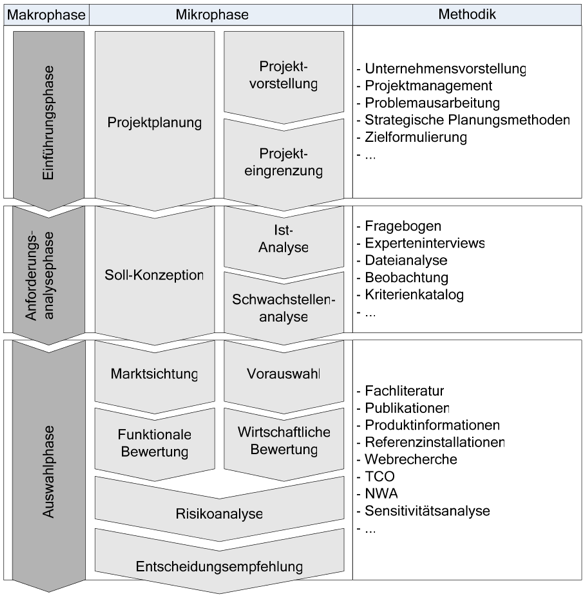
\includegraphics[width=10.629cm,height=10.781cm]{INMEA5BeckmannMarco-img001.png} \par}
{\centering\sffamily
Abb. 1: Vorgehensmodell für Software-Migrationen nach [Rog12]
\par}


\bigskip

{\sffamily
Das in Abb. 1 ersichtliche Vorgehensmodell beschreibt die verschiedenen, notwendigen Phasen, die einer Migration
vorausgehen. Die Genauigkeit dieser Planung ist hierbei maßgeblich für den späteren Erfolg der Migration. Im Rahmen
dieser Ausarbeitung wurde beispielsweise die in der Abbildung ersichtliche Methodik des Experteninterviews angewandt,
um Grundlagen für die Ist-Analyse zu erhalten.}


\bigskip

{\sffamily
In der Auswahlphase sind hierbei strategische, rechtliche und wirtschaftliche Aspekte zu berücksichtigen, ebenso wie der
spätere Systembetrieb, die notwendigen organisatorischen Aspekte und Anforderungen an die Sicherheit der Systeme. Nach
der Entscheidungsempfehlung werden dann eine oder mehrere Migrationsstrategien für die Einführung der neuen und die
Ablösung der alten Software festgelegt.}


\bigskip

\subsubsection[4.1.3.2 Migrationsstrategien]{\textbf{4.1.3.2 Migrationsstrategien}}

\bigskip

{\sffamily
Die Wahl der Migrationsstrategie ist jeweils fallbezogen zu prüfen. Es ist auch denkbar, für verschiedene Systeme
verschiedene Strategien zu nutzen. Nachfolgend werden auszugweise durch [Nüt14] beschriebene Migrationsstrategien
aufgeführt, welche in Punkt 4.1.4 hinsichtlich der Verwendung durch die Migrationsbeispiele der Hochschule beleuchtet
werden.}


\bigskip

{\sffamily
Big Bang Approach (Cold Turkey Strategy):}


\bigskip

{\sffamily
Hierbei wird das Altsystem von Grund auf neu entwickelt und zu einem bestimmten Zeitpunkt zur Verfügung gestellt.}


\bigskip

{\sffamily
Database First Approach / Database Last Approach:}


\bigskip

{\sffamily
Bei dieser Strategie wird erst das Datenbankmanagementsystem (Database First) migriert und anschließend alle
Applikationen und Schnittstellen in ein neues System überführt. Database Last beschreibt hierbei den genau umgekehrten
Vorgang.}


\bigskip

{\sffamily
Composite Database Approach:}


\bigskip

{\sffamily
Das neue Anwendungssystem wird schrittweise implementiert, während das Altsystem noch in Betrieb ist.}


\bigskip

{\sffamily
Chicken-Little Strategy:}


\bigskip

{\sffamily
Als Erweiterung des Composite Datebase Approach werden im Rahmen dieser Strategie zusätzliche Gateways entwickelt,
welche für die Überführung der Daten aus dem Altsystem in das Zielsystem verantwortlich zeichnen.}


\bigskip

{\sffamily
Butterfly Methodology:}


\bigskip

{\sffamily
Hierbei geht es um eine reine Datenmigration, bei der eine Kooperation zwischen Alt- und Neusystem nicht notwendig ist.
\ Die Entwicklung des neuen Systems wird also von der Migration der Daten separiert.}

\subsection{4.1.4 Migrationsbeispiele}

\bigskip

{\sffamily
Die Hochschule Emden/Leer nutzt derzeit für Ihren Internetauftritt das Enterprise Content Management System TYPO3 in der
Version 4.5. Die Dokumentenverwaltungssoftware Alfresco wird derzeit noch nicht genutzt. }


\bigskip

{\sffamily
Die folgenden Beispiele behandeln eine mögliche Migration von TYPO3 auf eine aktuelle Version inkl. Erstellung eines
responsive Designs, sowie die Neueinführung von Alfresco. Da die aktuelle Version von Alfresco auch die Möglichkeit
bietet Web Content zu verwalten, wäre theoretisch auch eine Migration des derzeitigen Internetauftritts in ein neu
eingeführtes Alfresco-System denkbar.}

\subsubsection[4.1.4.1 Responsive Website TYPO3]{\textbf{4.1.4.1 Responsive Website TYPO3}}
{\sffamily
TYPO3\footnote{\ http://typo3.org/typo3-cms/overview/ abgerufen am 28.05.2015} ist ein Open Source Enterprise Content
Management System zur Verwaltung webbasierter Inhalte. Es ist multilingual, hoch skalierbar und bietet ein aktives
Sicherheitsmanagement.}


\bigskip

{\sffamily
4.1.4.1.1 Ist-Zustand}


\bigskip

{\sffamily
Die Hochschule Emden/Leer nutzt derzeit ein TYPO3-Sytem in der Version 4.5 LTS (Long Term Support). Das System ist
derzeit noch nicht für die Anforderungen mobiler Endgeräte (responsive Design) gerüstet. Es werden verschiedene
Extensions von TYPO3 genutzt, möglicherweise auch eigens für die Hochschule entwickelte Extensions. Mitarbeiter und
Studenten sind als Benutzer innerhalb des CMS angelegt und können sich in einen geschützten Bereich über die Extension
FE-Login anmelden.}


\bigskip

{\sffamily
Für die derzeit eingesetzte Version von TYPO3 gibt es keinen Support mehr, so dass – weder für den TYPO3-Kern, noch für
die Extensions – neue Sicherheitspatches zur Verfügung gestellt werden. Dies stellt ein Sicherheitsrisiko für die
Hochschule dar. Allein aus diesem Grund sollte eine Migration auf ein aktuelles System erwogen werden. Ferner nutzt ein
Großteil der Besucher mobile Endgeräte, die aktuell nicht unterstützt werden.}


\bigskip

{\sffamily
4.1.4.1.2 Soll-Zustand}


\bigskip

{\sffamily
Das neue System soll über folgende Merkmale verfügen:}


\bigskip

\liststyleWWviiiNumvi
\begin{itemize}
\item {\sffamily
lange Support-Zeit, damit Sicherheitspatches eingespielt werden können}
\item {\sffamily
Unterstützung von mobilen Endgeräten}
\item {\sffamily
Übernahme bestehender Extensions oder Vorhandensein von Alternativen hierzu}
\item {\sffamily
Barrierefreiheit, damit auch Benutzer mit Handicap den Internetauftritt besuchen können}
\item {\sffamily
Suchmaschinenoptimierung (SEO)}
\item {\sffamily
Anbindung an die Benutzerverwaltung (Single-Sign-On) der Hochschule (bereits realisiert)}
\end{itemize}

\bigskip

{\sffamily
Hierzu wird zunächst ein strategisch günstiger Migrationsplan erstellt.}


\bigskip

{\sffamily
4.1.4.1.3 Migrationsplan}


\bigskip

{\sffamily
Um einen möglichst langen Supportzeitraum zu gewährleisten ist die Verwendung einer LTS-Version (Long Term Support)
anzuraten. Die derzeit aktuelle Version ist 6.2.12 LTS (Stand 27.05.2015), welche noch bis Ende März 2017 supportet
wird.}


\bigskip

{\sffamily
Derzeit ist bereits die Version 7.2.0 verfügbar, allerdings noch nicht als LTS-Version. Diese ist für Herbst 2015
avisiert. }


\bigskip

{\sffamily
Da die Migration einige Zeit in Anspruch nehmen wird, ist es sinnvoll, direkt auf die Version 7.x LTS zu migrieren, da
diese dann verfügbar sein wird. Hierfür sind allerdings Zwischenschritte vorzusehen, da eine direkte Migration von
Version 4.5 auf 7.x nicht möglich ist\footnote{\ http://wiki.typo3.org/Upgrade abgerufen am 28.05.2015}. Es muss
zunächst eine Migration auf die Version 6.2 LTS und von dort auf die Version 7.x erfolgen. Nachfolgend wird somit von
einer Migration auf die Version 7.x LTS ausgegangen.}


\bigskip

{\sffamily
Vor der Migration ist eine Überprüfung aller derzeit genutzten Extensions erforderlich. Dabei muss geprüft werden, ob
diese in der neuen Version noch gültig und lauffähig sind. Ist dies nicht der Fall, müssen Alternativen gesucht werden
und deren Realisierung in die Planung einfließen. Insbesondere selbst geschriebene Extensions müssen hinsichtlich der
Lauffähigkeit überprüft und ggf. ein Konzept zur Anpassung erstellt werden.}


\bigskip

{\sffamily
4.1.4.1.3.1 Hardwareanforderungen}


\bigskip

{\sffamily
Für eine erfolgreiche Migration sind bestimmte Hardwareanforderungen Voraussetzung. Unter anderem muss mindestens PHP
5.5, MySQL 5.5 und mehr als 200 MB freier Plattenplatz zur Verfügung stehen. Die genauen Konfigurationseinstellungen
inkl. allen benötigten Module sind den
Installationsvorgaben\footnote{\ https://github.com/TYPO3/TYPO3.CMS/blob/master/INSTALL.md abgerufen am 28.05.2015} der
TYPO3 Association zu entnehmen.}


\bigskip

{\sffamily
4.1.4.1.3.2 Entwicklungssystem}


\bigskip

{\sffamily
Zur Realisierung des neuen Systems wird ein Entwicklungssystem mit den oben beschriebenen Hardwareanforderungen
aufgesetzt. Über einen Dump der Datenbank werden die Daten des Produkivsystems in die Datenbank des Entwicklungssystems
übertragen. Das gesamte Dateisystem des TYPO3-Produktivsystems wird ebenfalls auf das Entwicklungssystem übertragen.
Dort werden dann die Konfigurationseinstellungen von TYPO3 angepasst, damit ein identisches, lauffähiges System
ensteht.}


\bigskip

{\sffamily
Innerhalb dieses Systems erfolgt die Migration auf die verschiedenen Versionen, die Anpassung der Extensions und die im
Rahmen der Migration notwendige Softwareentwicklung.}


\bigskip

{\sffamily
4.1.4.1.3.3 Migration}


\bigskip

{\sffamily
Im Rahmen der Migration müssen Softwaretechnisch folgende Punkte berücksichtigt werden:}


\bigskip

\liststyleWWviiiNumiv
\begin{itemize}
\item {\sffamily
Migration des TYPO3-Kerns}
\item {\sffamily
Migration aller eingesetzten Extensions}
\item {\sffamily
Anpassung selbstgeschriebener Extensions}
\item {\sffamily
Umstellung des Layout-Konzeptes von TYPO3 (von derzeit wahrscheinlich Templa-Voilà) auf Fluid-Templating}
\item {\sffamily
Schaffung einer Basis für responsive Design, beispielsweise auf Basis des Frameworks Bootstrap}
\item {\sffamily
Erweiterung / Anpassung der TypoScript-Programmierung}
\item {\sffamily
Anpassung Menüprogrammierung (TypoScript und Template)}
\item {\sffamily
Neuerstellung benötigter Fluid-Templates auf Basis von Haupttemplates und Partials}
\item {\sffamily
Programmierung eigener Extensions, falls notwendig}
\end{itemize}

\bigskip

{\sffamily
4.1.4.1.3.4 Produktivsetzung}


\bigskip

{\sffamily
Die Ablösung des derzeitigen Systems erfolgt anhand der Migrationsstrategie Big Bang Approach, da mit dem
Entwicklungssystem ein fertig entwickeltes und hinsichtlich des Datenbestandes aktuelles System zur Verfügung steht.
Die Produktivsetzung erfolgt in umgekehrter Reihenfolge wie die Einrichtung des Entwicklungssystems, also mit
Datenbank-Dump, Datei-Migration und ggf. TYPO3-Konfigurations-anpassungen. Hierdurch ist die Downtime für den
Internetauftritt der Hochschule Emden minimal.}


\bigskip


\bigskip


\bigskip


\bigskip


\bigskip


\bigskip


\bigskip


\bigskip


\bigskip


\bigskip


\bigskip


\bigskip


\bigskip


\bigskip


\bigskip


\bigskip


\bigskip


\bigskip


\bigskip


\bigskip


\bigskip

{\sffamily
\textbf{4.1.4.2 Alfresco}}


\bigskip

{\sffamily
Alfresco\footnote{\ https://www.alfresco.com/de/solutions/document-management abgerufen am 28.05.2015} ist ein
Dokumenten-Management-System welches als Open-Source-Plattform offene Standards unterstützt. Hiermit lässt sich der
gesamte Content auf einer einzelnen Plattform konsolidieren und damit die Benutzerfreundlichkeit erhöhen und die Kosten
senken.}


\bigskip

 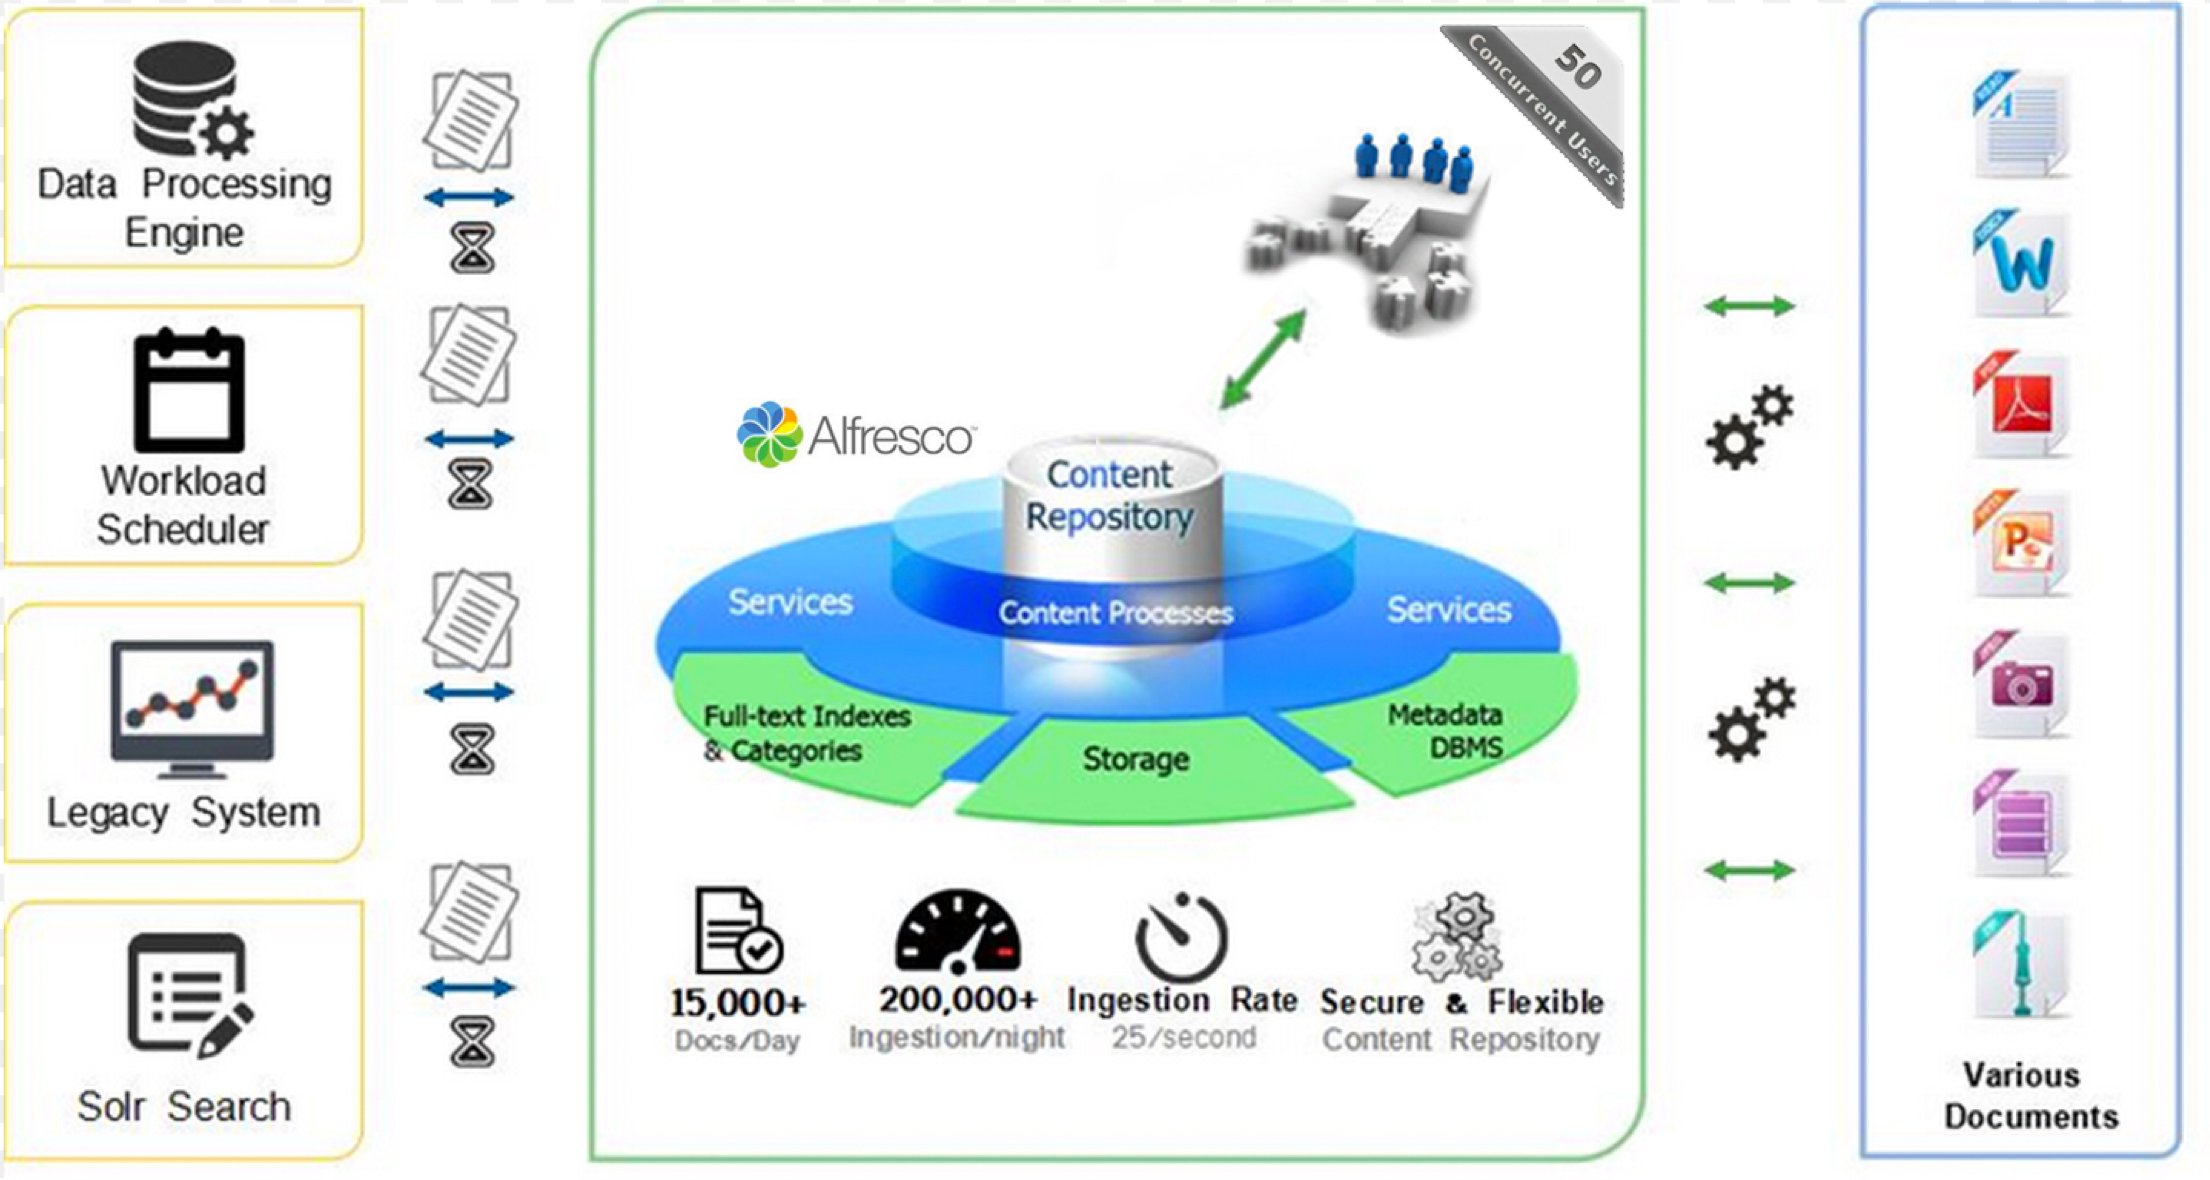
\includegraphics[width=14.215cm,height=7.588cm]{INMEA5BeckmannMarco-img002.png} 

{\centering\sffamily
Abb. 2: Übersicht Alfresco nach [Cab14]
\par}


\bigskip

{\sffamily
Peter Franke – Leiter des Rechenzentrums der Hochschule Braunschweig/Wolfenbüttel – berichtet in [Fra11] von positiven
Erfahrungen seit der Einführung von Alfresco.}


\bigskip

{\sffamily
4.1.4.2.1 Ist-Zustand}


\bigskip

{\sffamily
Alfresco wird derzeit von der Hochschule Emden/Leer noch nicht eingesetzt. Derzeit werden Dokumente in verschiedensten
Systemen verwaltet und zugänglich gemacht. Auszugsweise sind hier zu nennen:}


\bigskip

\liststyleWWviiiNumviii
\begin{itemize}
\item {\sffamily
Austauschlaufwerke für Dozenten}
\item {\sffamily
Webseiten mit offenen und geschlossenen Bereichen (Kennzahlen, Daten, Fakten für Mitarbeiter und Dekane)}
\item {\sffamily
Eigene Software Vorlesungsverzeichnis im Fachbereich Seefahrt}
\item {\sffamily
Software EvaSys für die Evaluierung}
\item {\sffamily
Gigamove zum Austausch großer Datenmengen}
\item {\sffamily
Eigene Systeme in den Fachbereichen (Labor)}
\end{itemize}

\bigskip

{\sffamily
Derzeit gibt es also viele gewachsene Systeme und Strukturen}


\bigskip

{\sffamily
4.1.4.2.2 Soll-Zustand}


\bigskip

{\sffamily
Das neue System soll über folgende Merkmale verfügen:}


\bigskip

\liststyleWWviiiNumvii
\begin{itemize}
\item {\sffamily
Migration aller vorhandener Dokumente auf das neue System für eine zentrale Verwaltung}
\item {\sffamily
Versionsmanagement}
\item {\sffamily
Schneller Zugriff}
\item {\sffamily
Ortsunabhängiger Zugriff}
\item {\sffamily
Verwaltung verschiedenster Dokumenttypen}
\item {\sffamily
Keine Client-Installation notwendig}
\end{itemize}

\bigskip

{\sffamily
Die Software Alfresco bietet alle diese Merkmale. In der aktuellen Version wird auch die Auslieferung von Web-Content
unterstützt, so dass für die Zukunft auch eine Migration des Internetauftritts in das Alfresco-System denkbar wäre.
Alternativ könnte Alfresco auch im Rahmen des Single Source Publishing Konzeptes als Content-Quelle für das
TYPO3-System genutzt werden. Die Berliner Philharmoniker nutzen bereits dieses Konzept, wie aus einer Case
Study\footnote{\ http://www.form4.de/artikel/alfresco-meets-typo3/ abgerufen am 28.05.2015} der Firma form4 GmbH
hervorgeht. }


\bigskip

{\sffamily
Hinsichtlich des Dokumenten-Managements wird zunächst ein strategisch günstiger Migrationsplan zur Einführung von
Alfresco erstellt. Dabei muss auch die Entscheidung getroffen werden, welche Edition von Alfresco sinnvoll für die
Hochschule ist.}


\bigskip

{\sffamily
4.1.4.2.3 Migrationsplan}


\bigskip

{\sffamily
Da nach der Migration alle Dokumente zentral verwaltet werden, erscheint es sinnvoll, Alfresco als hochverfügbaren
Cluster auszulegen. Gegebenenfalls ist auch der Einsatz eines SAN (Storage Area Networks) mit räumlich getrennten
Speichereinheiten und entsprechend angepasstem Backup- und Restore-Konzept in Erwägung zu ziehen.}


\bigskip

{\sffamily
Grundsätzlich stehen von Alfresco die kostenlose Community Edition und die kostenpflichtige Enterprise Edition zur
Verfügung. Ein Vergleich der beiden Editionen findet sich auf der
Website\footnote{\ https://www.alfresco.com/de/alfresco-community-edition abgerufen am 28.05.2015} von Alfresco.}


\bigskip

{\sffamily
Folgt die IT-Leitung dem Vorschlag einer hochverfügbaren Realisierung, muss die Enterprise Edition eingesetzt werden, da
nur sie die Möglichkeit des Clusterings bietet. Hierbei ergibt sich der Vorteil, dass für diese Edition Support seitens
des Herstellers geboten wird und die wichtige Frage nach Service Level Agreements (SLA) damit gelöst werden kann.
Zusätzlich gibt es Zertifizierungsschulungen für Entwickler und Administratoren, welche im Rahmen des Change
Managements sinnvoll sind.}


\bigskip

{\sffamily
Das Alfresco-System wird komplett neu aufgesetzt und die (derzeit) auf verschiedenen Systemen verteilten Dokumente
werden nach und nach in das Alfresco-System migriert.}


\bigskip

{\sffamily
4.1.4.2.3.1 Hardwareanforderungen}


\bigskip

{\sffamily
Die Hardwareanforderungen richten sich stark nach den in Alfresco genutzten Modulen, bzw. ob die Community oder
Enterprise-Edition genutzt wird. Detailliert Hardwareanforderungen können nach Festlegung der Edition in der
Alfresco-Dokumentation\footnote{\ http://docs.alfresco.com/5.0/concepts/ha-intro.html abgerufen am 28.05.2015}
eingesehen werden. }


\bigskip

{\sffamily
Die Hardwareanforderungen sind unter anderem abhängig von:}


\bigskip

\liststyleWWviiiNumii
\begin{itemize}
\item {\sffamily
dem benötigten Anwendungsfall (welche Komponenten genutzt werden)}
\item {\sffamily
der Anzahl der gleichzeitig zugreifenden Benutzer}
\item {\sffamily
dem Speicherort der Dokumente}
\item {\sffamily
dem Betrieb im Rahmen einer Hochverfügbarkeitslösung}
\item {\sffamily
dem Einsatz von Load Balancern}
\item {\sffamily
dem Einsatz dedizierter Transformation Server}
\item {\sffamily
der Nutzung von Clustern für zu nutzende Interfaces}
\item {\sffamily
dem Einsatz von Caching-Verfahren}
\end{itemize}

\bigskip

 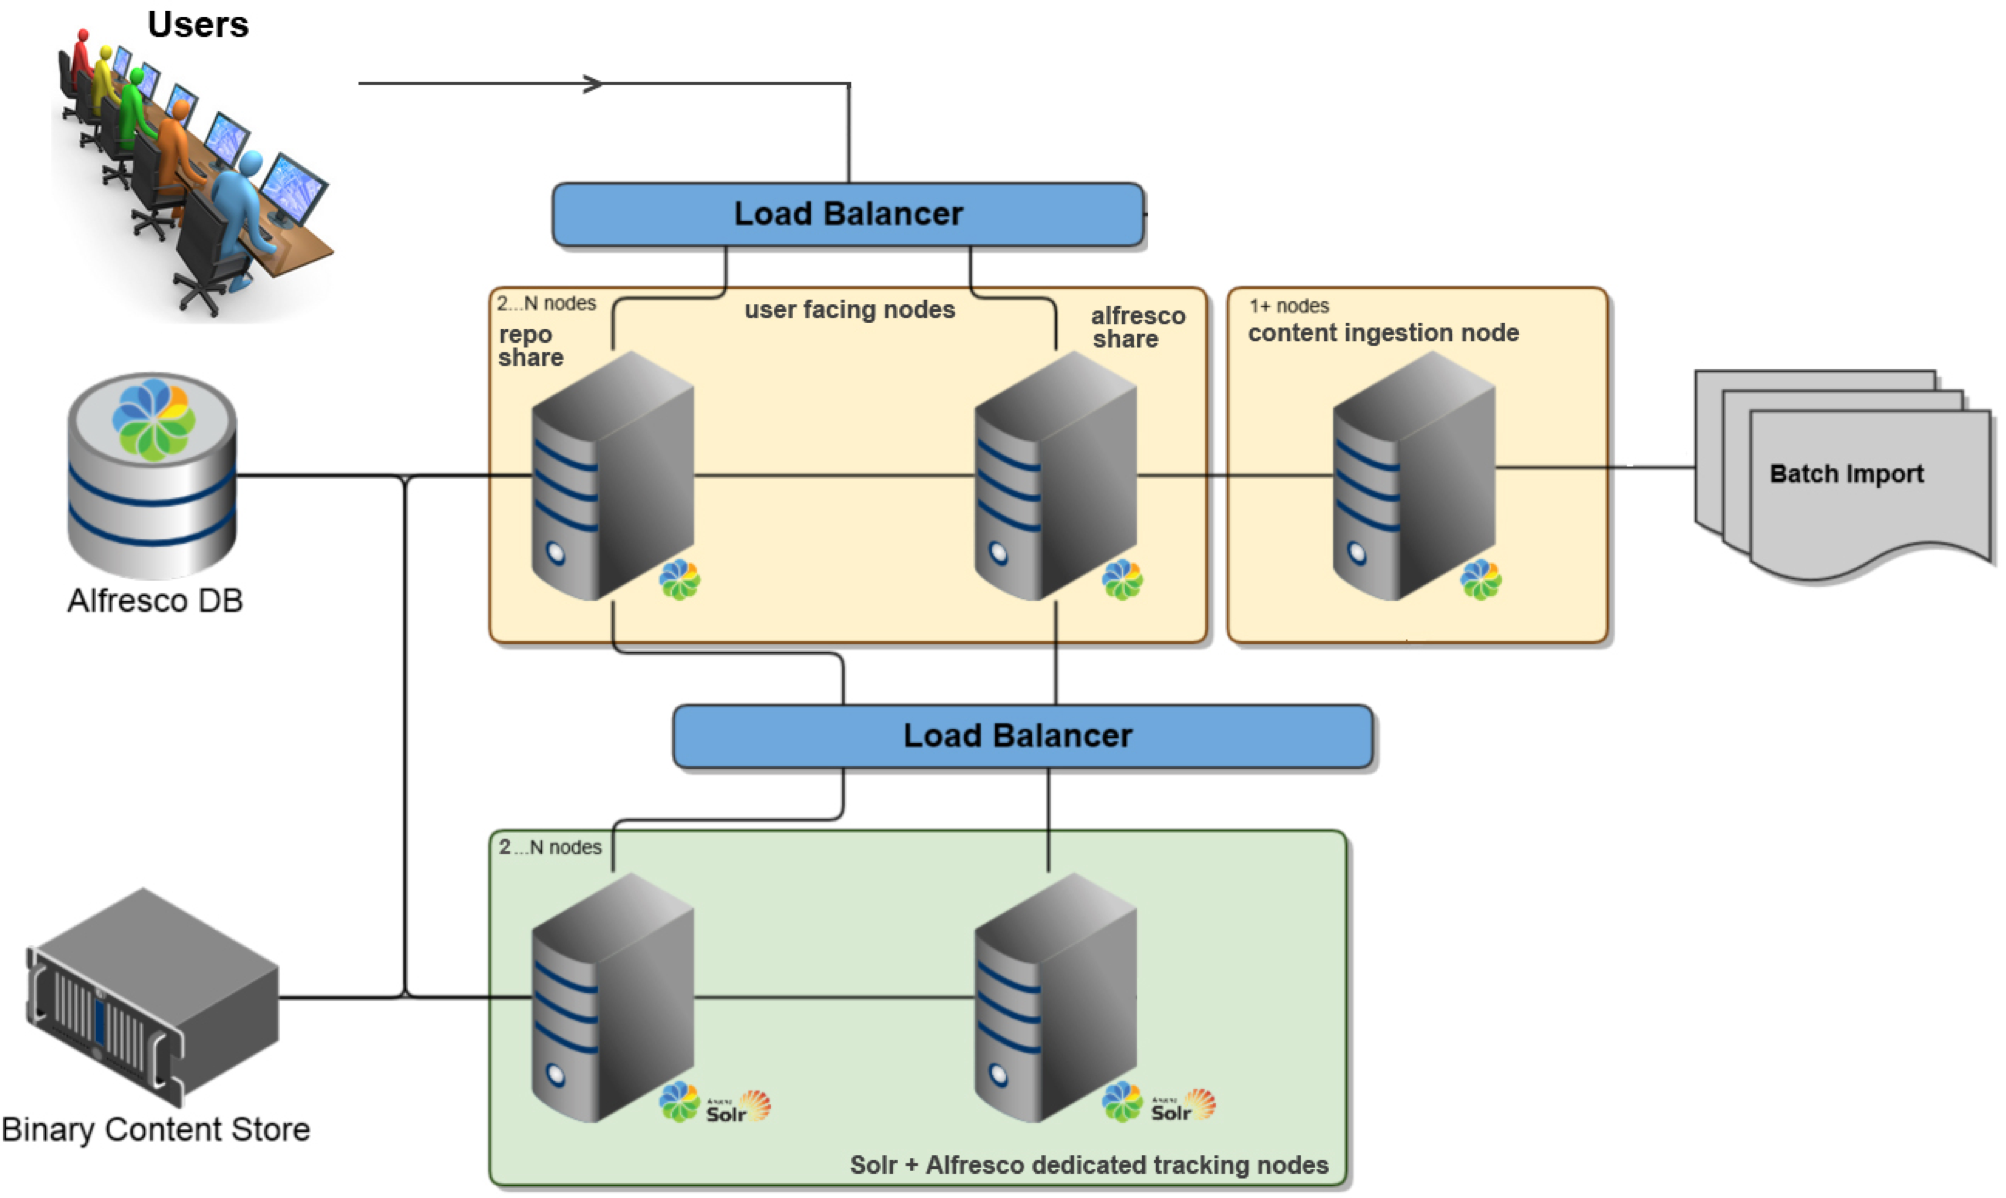
\includegraphics[width=14.605cm,height=8.724cm]{INMEA5BeckmannMarco-img003.png} 

{\centering\sffamily
Abb. 3: Mögliche Hardwarstruktur für Alfresco nach [Cab14]
\par}


\bigskip

{\sffamily
Abbildung 3 visualisiert hier eine mögliche Hardwarestruktur für ein Alfresco-System. }


\bigskip

{\sffamily
4.1.4.2.3.2 Entwicklungssystem}


\bigskip

{\sffamily
Das Entwicklungssystem wird nach den benötigten Hardwareanforderungen aufgesetzt. Hierauf erfolgt die Implementierung
von Alfresco inkl. den bei Bedarf benötigten Schnittstellen. Nach Fertigstellung kann das Entwicklungssystems direkt
als Produktivsystem genutzt werden, da die Datenmigration anschließend erfolgt, wie im folgenden Abschnitt
beschrieben.}


\bigskip

{\sffamily
4.1.4.2.3.3 Migration}


\bigskip

{\sffamily
Für die Migration bietet sich in diesem Fall die Migrationsstrategie Butterfly Methodology an, da hierbei nach und nach
die verschiedenen Altsysteme in das neue System überführt werden können. Da es sich beim Entwicklungssystem um ein
{\textquotedbl}leeres{\textquotedbl} System handelt, wird es nach Fertigstellung als Produktivsystem genutzt. Hierin
erfolgt dann nach und nach die Migration der Dokumente aus den unterschiedlichen Altsystemen.}


\bigskip

{\sffamily
4.1.4.2.3.4 Produktivsetzung}


\bigskip

{\sffamily
Wie bereits oben beschrieben, erfolgt die Produktivsetzung direkt nach Abnahme des Entwicklungssystem und erfolgt durch
dessen Übernahme. }


\bigskip


\bigskip

\clearpage
\bigskip

{\sffamily\bfseries
Literaturverzeichnis}

\begin{figure}
\centering
\begin{minipage}{2.54cm}
{\raggedleft\sffamily
I
\par}
\end{minipage}
\end{figure}
\begin{figure}
\centering
\begin{minipage}{7.938cm}
{\sffamily
Verzeichnisse}
\end{minipage}
\end{figure}

\bigskip

\begin{flushleft}
\tablefirsthead{}
\tablehead{}
\tabletail{}
\tablelasttail{}
\begin{supertabular}{m{1.6999999cm}m{13.269cm}}
{\sffamily \textbf{[Rog12]}} &
{\sffamily \textbf{Rogall-Grothe, Cornelia, 2012. }\textit{Migrationsleitfaden - Leitfaden für die Migration von
Hardware und Software.} Berlin: Die Beauftragte der Bundesregierung für Informationstechnik, 2012. -
http://www.cio.bund.de/SharedDocs/Publikationen/DE/Architekturen-und-Standards/migrationsleitfaden\_4\_0\_download.pdf?\_\_blob=publicationFile}

{\sffamily Abgerufen am 27.05.2015}\\
{\sffamily\bfseries [Cab14]} &
{\sffamily \textbf{Cabaceira, Luis, 2014. }\textit{Sizing your Alfresco platform},
\ http://de.slideshare.net/LuisCabaceira/sizing-your-alfrescoplatform}

{\sffamily Abgerufen am 27.05.2015}\\
{\sffamily\bfseries [Nüt14]} &
{\sffamily \textbf{Nüttgens, Markus, 2014. }\textit{Integration und Migration von IT-Systemen.} Universität Hamburg,
\ http://www.enzyklopaedie-der-wirtschaftsinformatik.de/wi-enzyklopaedie/lexikon/is-management/Integration-und-Migration-von-IT-Systemen/Ablosung-von-Altsystemen}

{\sffamily Abgerufen am 27.05.2015}\\
{\sffamily\bfseries [Fra11]} &
{\sffamily \textbf{Franke, Peter, 2011. }\textit{IT-Konzept.} Hochschule Braunschweig/Wolfenbüttel,
\ http://www.ostfalia.de/export/sites/default/de/rz/documents/it-konzept-2011.pdf}

{\sffamily Abgerufen am 27.05.2015}\\
{\sffamily\bfseries [BB10]} &
{\sffamily \textbf{Bode, Arndt, Borgeest, Rolf (Hrsg.), 2010. }\textit{Informationsmanagement in Hochschulen.}
Heidelberg: Springer-Verlag, 2010. - ISBN 978-3-642-04719-0}\\
{\sffamily\bfseries [Kna15]} &
{\sffamily \textbf{Knauer, Dirk, 2015. }\textit{Act Big - Neue Ansätze für das Informationsmanagement,
Informationsstrategie im Zeitalter von Big Data und digitaler Transformation. }Heidelberg: Springer-Verlag, 2015. -
ISBN \textstylepissn{978-3-658-06750-2}}\\
{\sffamily\bfseries [Her15]} &
{\sffamily \textbf{Herzfeldt, Alexander, 2015. }\textit{Untersuchung der Profitabilität von IT-Lösungen - Eine
Praxisstudie aus Anbietersicht. }Heidelberg: Springer-Verlag, 2015. - ISBN \textstylepissn{978-3-658-08854-5}}\\
{\sffamily\bfseries [Hub14]} &
{\sffamily \textbf{Huber, Sebastian, 2014. }\textit{Informationsintegration in dynamischen Unternehmensnetzwerken -
Architektur, Methode und Anwendung. }Heidelberg: Springer-Verlag, 2014. - ISBN \textstylepissn{978-3-658-07747-1}}\\
{\sffamily\bfseries [BF11]} &
{\sffamily \textbf{Breiter, Andreas, Fischer, Arne, 2011. }\textit{Implementierung von IT-Service-Management -
Erfolgsfaktoren aus nationalen und internationalen Fallstudien. }Heidelberg: Springer-Verlag, 2011. - ISBN
\textstylepissn{978-3-642-18476-5}}\\
{\sffamily\bfseries [BBH+05]} &
{\sffamily \textbf{Bischof, C., Brett, W., Held, W., Lang, U., Lix, B., Oevel, G., Ziegler, H., 2005. }\textit{Die
Informations- und Kommunikationstechnische Infrastruktur und ihre mittelfristige Entwicklung an den Hochschulen des
Landes NRW II. }NRW: Arbeitskreis der Leiter Wissenschaftlicher Rechenzentren in NRW (ARNW), 2010.\textit{
}http://www.ARNW.de/docs/TIMEII - abgerufen am: 06.04.2015}\\
{\sffamily\bfseries [BBL07]} &
{\sffamily \textbf{Breitner, Michael, Bruns, Beate, Lehner, Franz, 2007. }\textit{Neue Trends im E-Learning - Aspekte
der Betriebswirtschaftslehre und Informatik. }Heidelberg: Springer-Verlag, 2007. - ISBN
\textstylepissn{978-3-7908-1917-5}}\\
{\sffamily\bfseries [BK10]} &
{\sffamily \textbf{Bröcker, Werner, König, Frank, 2010. }\textit{Informationsverarbeitung an Hochschulen - Organisation,
Dienste, Systeme. Empfehlungen der Kommission für IT-Infrastruktur für 2011-2015. }Bonn: Deutsche
Forschungsgemeinschaft, 2010. - http://www.dfg.de/wgi - abgerufen am: 06.04.2015}\\
\end{supertabular}
\end{flushleft}

\bigskip


\bigskip


\bigskip


\bigskip


\bigskip


\bigskip


\bigskip


\bigskip


\bigskip


\bigskip


\bigskip


\bigskip


\bigskip


\bigskip


\bigskip


\bigskip


\bigskip


\bigskip


\bigskip


\bigskip


\bigskip


\bigskip


\bigskip


\bigskip


\bigskip


\bigskip


\bigskip


\bigskip


\bigskip


\bigskip


\bigskip


\bigskip


\bigskip


\bigskip


\bigskip


\bigskip


\bigskip


\bigskip


\bigskip


\bigskip


\bigskip

{\sffamily\bfseries
Abbildungsverzeichnis}


\bigskip

\begin{flushleft}
\tablefirsthead{}
\tablehead{}
\tabletail{}
\tablelasttail{}
\begin{supertabular}{m{2.213cm}m{1.7049999cm}m{10.729cm}}
{\sffamily Abbildung 1} &
~
 &
~
\\
{\sffamily Abbildung 2} &
~
 &
~
\\
{\sffamily Abbildung 3} &
~
 &
~
\\
{\sffamily Abbildung 4} &
~
 &
~
\\
\end{supertabular}
\end{flushleft}

\bigskip


\bigskip


\bigskip


\bigskip
\end{document}
